\documentclass[a4paper,10.5pt,twoside]{article}%方框内设置默认的正文字体大小
%基于北京航空航天大学仪器科学与光电工程学院实验报告及课程报告排版得来,类似于毕业论文排版格式
%后续将更新毕业论文排版格式
\usepackage{graphicx,float}%使用图的宏包,使用图的浮动体宏包,引入参数H使图像紧跟当前文字
\usepackage{caption} %使用图表标题的宏包
\usepackage[colorlinks=true,pdfstartview=FitH,%
linkcolor=black,anchorcolor=violet,citecolor=magenta]{hyperref}%加载hyperref宏包,使用超链接
\usepackage{setspace}%用于设置行间距列间距等命令的宏包
\usepackage{array}%设置列表高度宽度的宏包
\usepackage{zhnumber}%使用中文数字编号的宏包
\usepackage{titlesec,titletoc}%使用标题自定义形式的宏包和使用目录自定义形式的宏包
\usepackage{siunitx}%物理学单位宏包
\usepackage{tabularx}%让表格宽度等于页面宽度
\usepackage{makecell}%单个表格单元调整的宏包
\usepackage{subfigure} %%使用子图的宏包
\usepackage[backend=biber,bibstyle=gb7714-2015,%nature,%%加载biblatex宏包,使用参考文献
citestyle=gb7714-2015%,backref=true%%其中后端backend使用biber
,url=false,doi=false
]{biblatex}%标注(引用)样式citestyle,著录样式bibstyle都采用gb7714-2015样式
% \usepackage{pgfplots}%类似tikz的一个画图库,主要画统计图
\usepackage{../customStyle}
% \usepackage[lite,subscriptcorrection,slantedGreek,nofontinfo]{mtpro2}%使用mathtimepro2商业字体作为数学环境,并不推荐

%biblatex宏包的参考文献数据源加载方式,注意book.bib应当与.tex文件在同一目录下,不然有可能会报错
\addbibresource[location=local]{book.bib}
%%% 下面的命令重定义页面边距,使其符合中文刊物习惯 %%%%
\setlength{\oddsidemargin}{0.63cm}  % 3.17cm - 1 inch
\setlength{\evensidemargin}{\oddsidemargin}
% 重定义页眉
\pagestyle{beihang}
\fancyhead[CO]{机电仿真实验报告}%

\graphicspath{{./fig}}

\begin{document}
{
  %% ----------- 封面部分 ------------ %%
\pagestyle{empty}
\begin{figure}
  
\includegraphics{title.jpg}
\end{figure}
\begin{center}

  \begin{figure}[h]

    \centering
    
\includegraphics[]{title.png}\par
    \vspace{4em}
    \large{\chuhao\heiti{机电仿真实验}}\par
    \vspace{6em}
  \end{figure}

  
  \large{\yihao\heiti{Labwindows/CVI实验报告}}\par
  \vspace{8em}

  \begin{spacing}{2.0}
    \begin{tabular}{cc}


      {\xiaosanhao\heiti{学\quad 院\quad 名\quad 称}} & {\xiaosanhao\heiti{\dlmu{仪器科学与光电工程学院}}}    \\
      {\xiaosanhao\heiti{学\quad \quad\quad\quad\quad 号}} & {\xiaosanhao\heiti{\dlmu{SY2317301} }} \\
      {\xiaosanhao\heiti{姓\quad \quad\quad\quad\quad 名}} & {\xiaosanhao\heiti{\dlmu{陈博非} }}       \\
    \end{tabular}
  \end{spacing}
\end{center}
\begin{center}
  {\xiaoerhao\heiti{\now}}
\end{center}

\thispagestyle{empty}
}

\newpage
%% ----------- 封面部分结束 ------------ %%


%% ----------- 目录部分 ------------ %%
% \pagenumbering{roman}

% \setcounter{tocdepth}{3}
% %设定目录深度                      
% \tableofcontents
% %列出目录
% \newpage
%% ----------- 目录部分结束 ------------ %%
\pagenumbering{arabic}
\setcounter{page}{1}

\section{实验背景}
测试系统的静态特性就是指当被测量$x$不随时间变化或随时间的变化程度远缓慢于系统固有的最低阶运动模式的变化速度时,测试系统的输出量$y$与输入量$x$之间的函数关系。测试系统的静态特性,是通过静态标定的过程获取的。
\subsection{线性度}
一般情况下,要求传感器具有线性特性,但传感器的实际特性却是非线性的曲线,这种实际特性曲线与基准直线间的偏差称为非线性误差。传感器的非线性误差指标通常用线性度表示,线性度的定义为:
\begin{equation*}
  e_L= \frac{\abs{\Delta L_\mathrm{max}}}{y_\mathrm{FS}} \times 100\%
\end{equation*}\par
式中,$e_L$表示线性度(非线性误差),$\abs{\Delta L_\mathrm{max}}$表示在整体测量范围内绝对值最大的非线性误差,$y_\mathrm{FS}$表示传感器的满量程输出值。由定义可知,传感器的线性度是以基准直线为参考的,实际测量中采用的是最小二乘线性度。
\subsection{重复性}
在相同的工作条件下,在一段短的时间间隔内,输入量从同一方向作满量程变化时,同一输入量值所对应的多次测量所得到的一组输出量值,他们之间的相互偏离的程度便称为传感器的重复性。当传感器在全量程范围内多次重复测试时,同是正行程或同是反行程上对应同一输入量,其输出量之间的差值称为重复性偏差。正、反行程的重复性偏差分别为:
\begin{align}
  \Delta R^{(c)}_j &= \max\curlbrac{y_j^{(c)}} - \min\curlbrac{y_j^{(c)}}\\
  \Delta R^{(f)}_j &= \max\curlbrac{y_j^{(f)}} - \min\curlbrac{y_j^{(f)}}
\end{align}\par
在全量程内,重复性偏差的绝对值 的最大值与基准直线上满量程输出之比称为重复性误差,定义如下:
\begin{equation*}
  e_L= \frac{\abs{\Delta R_\mathrm{max}}}{y_\mathrm{FS}} \times 100\%
\end{equation*}\par
\section{实验数据}
现有两个虚拟传感器的标定数据,分别存储为a.cld和b.cld两个文件中,其数据定义为结构体CalibrateData,声明如下:
\begin{lstlisting}[language=C]
  typedef struct CalibrateData{
    int    inputnum;               //输入测量点数
    double *input;                 //输入测量点的值,数据长度为inputnum
    char   inputunit[10];          //输入物理量的单位
    int    roundnum;               //测量的循环数
    char   outputunit[10];         //测量所得物理量的单位
    double *output;                //测量的值,其排列顺序为:
                                   //第一循环正行程,第一循环反行程,
                                   //第二循环正行程,第二循环反行程,
                                   //以此类推。数据长度为inputnum*2*roundnum
  } CALIDATA;
\end{lstlisting}
% \begin{figure}[H]
%   \centering
%   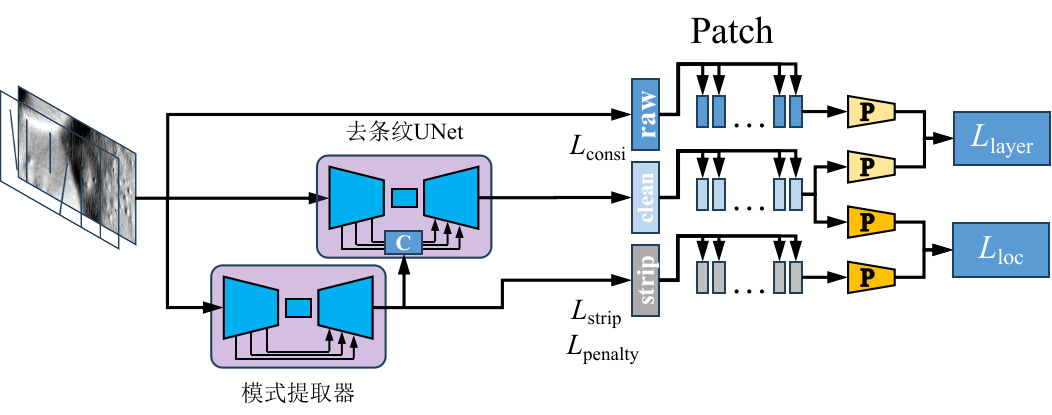
\includegraphics[width=0.8\textwidth]{workflow.png}
%   \caption{检测算法工作流程}
%   \label{fig:workflow}
% \end{figure}
\subsection{数据加载环节}

\subsection{扩散网络环节}

\subsection{后处理环节}

\section{算法原理}

\section{程序设计流程与说明}
\newpage
\section{实验结果与分析}
\newpage
\section{结论}

\newpage
\printbibliography[heading=bibliography,title=参考文献]
\end{document}
